\chapter{無線センサネットワークにおけるオペレーティングシステム}
\begin{large}
\begin{quote}
本章では,最初にセンサネットワークの一般公衆化を説明し,公衆センサデータ管理における必須な機能要件である地理的探索について述べる.次に,公衆センサデータ管理のシステム設計の際の重要な概念であるデータ管理の時間的密度を解説し,最後にセンサデータの時間的特殊性とそれに起因する公衆センサデータ管理の問題点を述べる.
%本章では,
\end{quote}
\end{large}
\clearpage


%\section{無線センサネットワークにおけるオペレーティングシステム}
%無線センサネットワークのオペレーティングシステムには主に2種類あり,
%イベントモデルとスレッドモデルが存在している.
%無線センサネットワーク用のオペレーティングシステムではイベントモデルが主流となっている.

\section{イベントモデル}
イベントモデルで構築されたオペレーティングシステムは全てのタスクをイベントによって起動し,
run-to-completion で実行する形態のオペレーティングシステムである.
イベントモデルは図\ref{fig:event_model}に示されるように,
ひとつのイベントループと多数のイベントハンドラから構成される.
イベントループはイベントの到着を待ち,
イベントが届くとイベントに関連付けられているイベントハンドラを実行する.
イベントモデルではイベント駆動型プログラミングによってアプリケーションが記述される.
イベントハンドラは寿命の短いrun-to-completionで記述され,
プリエンプションされることがない.
つまり,イベントモデルはタスクは関数呼び出しと等価であり,
実行ストリームがひとつで実現されるため各タスクでローカル変数の領域を共有可能であることから,
省資源かつ低オーバヘッドで並列性を実現できる.
また,各タスクが不可分に実行されるので共有資源に対する排他制御が不要となり,
安全性が高い.
さらに,CPU の特殊な機能を用いなくても実装できるので移植性も高い.
\begin{figure}[htbp]
 \begin{center}
  
\includegraphics[width=60mm]{./images/event_model.eps}
 \end{center}
 \caption{イベントモデル}
 \label{fig:event_model}
\end{figure}


%\subsection{TinyOS: An Operating System for Sensor Networks}
\subsection{TinyOS}
この中で代表的なものがTinyOS\cite{Hill:2000:SAD:356989.356998}\cite{Levis04tinyos:an}である.
TinyOSはカリフォルニア大学バークレー校のSmartDust Projectで開発されたオペレーティングシステムである.
現在無線センサネットワークの標準的なオペレーティングシステムとして扱われており,
Crossbow社から発売されているMica2やMicaZ\cite{Hill:2002:MWP:623308.624560},
Telos\cite{Polastre:2005:TEU:1147685.1147744},iMote\cite{Nachman:2005:IMP:1147685.1147760}上で動作する.
TinyOSはCPUの特別な機能を使用せずに実装可能であるため,移植性が高く,
ATMELのAVR128LやTexsusのMSP430,ARM7などさまざまなCPUに移植されている.
TinyOSのアーキテクチャを図\ref{fig:system_conf_of_tinyos}に示す.

\begin{figure}[htbp]
 \begin{center}
  \includegraphics[width=100mm]{./images/system_conf_of_tinyos.eps}
 \end{center}
 \caption{TinyOS アーキテクチャ}
 \label{fig:system_conf_of_tinyos}
\end{figure}

TinyOSではnesC\cite{Gay:2003:NLH:781131.781133}と呼ばれるイベント駆動型の新しい言語で
複数のイベントハンドラを1つのモジュールとして設計可能な機能を提供している.
図にnesC言語がコンパイルされて実行されるまでの流れを示す.
nesC言語はnesCコンパイラによってC言語のコードに変換された後,
Cコンパイラによって実行形式へと変換される.
nesC言語を採用することによって,
イベントモデルの持つプログラムの開発のし辛さを提供し,
新しい言語を学ばなければならないという手間がかかってしまうものの,
nesCはイベント駆動型に特化した最適化を行っているため省資源性を実現している.


%Earlier versions of TinyOS supported 
%a non-preemptive First-In-First-Out (FIFO) scheduling algorithm.
%Therefore, those versions of TinyOS do not support real-time application. 
%The core of the TinyOS execution model are tasks that run to completion in a FIFO manner.
%Since TinyOS supports only non preemptive scheduling, 
%task must obey run to completion semantics. 
%Tasks run to completion with respect to other task 
%but they are not atomic with respect to interrupt handlers, commands, and 
%events they invoke. 
%Since TinyOS uses FIFO scheduling, 
%disadvantages associated with FIFO scheduling are also associated with the TinyOS scheduler. 
%The wait time for a task depends on the task’s arrival time. 
%FIFO scheduling can be unfair to latter tasks especially 
%when short tasks are waiting behind longer ones.
%In [3], the authors claim that they have added support 
%for an Earliest Deadline First (EDF) scheduling algorithm in TinyOS, 
%to facilitate real-time applications. 
%The EDF scheduling algorithm does not produce a feasible schedule 
%when tasks content for resources. 
%Thus, TinyOS does not provide a solid real-time scheduling algorithm 
%if different threads content for resources. 

%TinyOS does not provide any explicit support for real-time applications. 
%As we already discussed in the scheduling section above, 
%tasks in TinyOS observe run to completion semantics in a FIFO manner, 
%hence in its original form, 
%TinyOS is not a good choice for sensor networks that are being deployed 
%to monitor real-time phenomena. 
%An effort has been made to implement an Earliest Deadline First (EDF) 
%process scheduling algorithm 
%and it has been made available in newer versions of TinyOS. 
%However, it has been shown that the EDF algorithm cannot produce a feasible schedule 
%when tasks content for resources. 
%In the nutshell, TinyOS is not a strong choice for real-time applications. 
%TinyOS does not provide any specific MAC, network, or transport layers protocol implementations
%that support Quality of Service requirements of real-time multimedia streams. 
%At the MAC layer, TinyOS supports TDMA, 
%which can be fine-tuned depending upon the requirements of an application 
%to support multimedia traffic streams.



%\subsection{A Dynamic Operating System for Sensor Nodes}
\subsection{SOS}
TinyOSがモノリシックなシステムイメージを持っていたのに対し,
SOS\cite{Han:2005:DOS:1067170.1067188}は
イベント駆動型オペレーティングシステムに動的モジュールの機能を実現したものである.
SOSではカーネルから動的モジュールをロードする時に関数の型チェックを行うことで
関数の型違反に伴うバグを防ぐ仕組みを取り入れている.




\section{スレッドモデル}\label{sec:threads_model}
%スレッドモデルを図 5 に示す.
スレッドモデルは図\ref{fig:threads_model}に示されるように,
複数のスレッドから構成され,
各スレッドはそれぞれ独立に実行ストリームを持っており,
低い優先度のスレッドは高い優先度のスレッドにプリエンプションされるという特徴を持つ.
スレッドモデルではユーザはあたかもCPUを占有しているかのように
一連の処理をひとつのスレッドとして記述することができるため,
プログラムが書きやすい.
また,プリエンプションを行うことも想定しているため,
ハードリアルタイム処理をサポートすることができる.
\begin{figure}[htbp]
 \begin{center}
  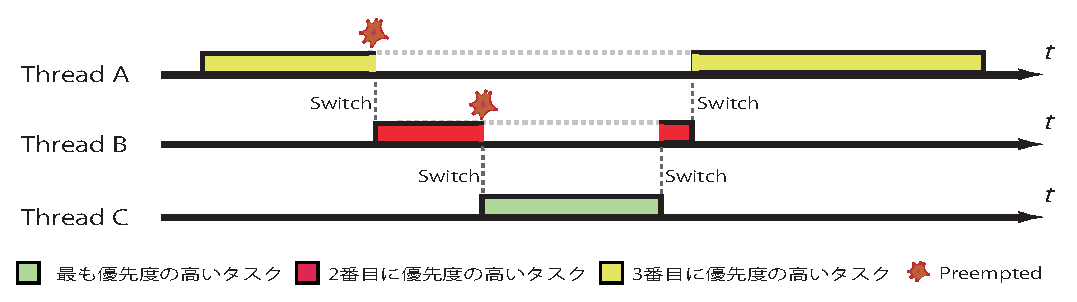
\includegraphics[width=140mm]{./images/threads_model.eps}
 \end{center}
 \caption{スレッドモデル}
 \label{fig:threads_model}
\end{figure}


%\subsection{Nano-RK: an Energy-aware Resource-centric RTOS for Sensor Networks}
\subsection{Nano-RK}
Nano-RK\cite{Eswaran:2005:NER:1106608.1106672}は,
無線センサネットワークにおけるマルチタスク処理機能を備えた
リアルタイムオペレーティングシステムであり,
%Nano-RK [31] is a fixed, preemptive multitasking real-time OS for WSNs. 
%Nano-RKを設計することで,
リソースの使用が制限された無線センサネットワークにおける,
マルチタスク処理,
優先度順位スケジューリングや
マルチホップネットワークのサポートを実現する.
%The design goals for Nano-RK are multitasking, support for multi-hop networking, 
%support for priority-based scheduling, 
%timeliness and schedulability, extended WSN lifetime, 
%application resource usage limits, and small footprint.
2KbのRAMと18KbのROMを使用し,
Rate Monotonic Scheduleingと
Rate Harmonized Scheduling\cite{Rowe:2008:RSS:1475690.1475895}を利用することによって,
ハードリアルタイムアプリケーションとソフトリアルタイムアプリケーションの
両方をサポートする.
%Nano-RK uses 2 Kb of RAM and 18 Kb of ROM. Nano-RK provides support for CPU, 
%sensors, and network bandwidth reservations.
%Nano-RK supports hard and soft real-time applications 
%by the means of different real-time scheduling algorithms, 
%e.g., rate monotonic scheduling and rate harmonized scheduling [32]. 
現在動作確認がとれているセンシングプラットフォームとして,
FireFly\cite{Rowe_firefly:a}と
MicaZ\cite{Hill:2002:MWP:623308.624560}が挙げられる.
Nano-RKのアーキテクチャは図\ref{fig:system_conf_of_nrk}のとおりである.
%Nano-RK provides networking support through socket-like abstraction. 
%Nano-RK supports FireFly [33] and MicaZ sensing platforms. 

\begin{figure}[htbp]
 \begin{center}
  \includegraphics[width=100mm]{./images/system_conf_of_nrk.eps}
 \end{center}
 \caption{Nano-RK アーキテクチャ}
 \label{fig:system_conf_of_nrk}
\end{figure}



%\subsection{MANTIS OS: An Embedded Multithreaded Operating System for Wireless Micro Sensor Platforms}
\subsection{MANTIS OS}
MANTIS OS\cite{Bhatti:2005:MOE:1160162.1160178}はLinuxやFreeBSDなどで
用いられているスレッドと同様の機能をセンサノード上で
実現したスレッドモデルのオペレーティングシステムである.
開発者はLinuxやFreeBSDなどで用いられているソフトウェアを
大きな変更無しにMANTIS OS上に移植することができる.
また,MANTIS OS上の1つのスレッドとして
TinyOS\cite{Hill:2000:SAD:356989.356998}\cite{Levis04tinyos:an}を
実装することも可能であり\cite{Trumpler06asystematic},
さまざまなソフトウェアリソースをMANTIS OS上で動作可能であることも特徴的である.
MANTIS OSはC言語で実装されており,
アプリケーション開発者もC言語を用いて開発を行うことが可能である.
図\ref{fig:system_conf_of_mantis}はMANTIS OSのアーキテクチャである.

%The MultimodAl system for NeTworks of In-situ wireless Sensors (MANTIS) provides 
%a new multithreaded operating system for WSNs.
%MANTIS is a lightweight and energy efficient operating system. 
%It has a footprint of 500 bytes, 
%which includes kernel, scheduler, and network stack. 
%The MANTIS Operating System (MOS) key feature is that 
%it is portable across multiple platforms, 
%i.e., we can test MOS applications on a PDA or a PC [28].
%Afterwards, the application can be ported to the sensor node.
%MOS also supports remote management of sensor nodes through dynamic programming. 
%MOS is written in C and it supports application development in C.
%The following subsections discuss the design features of MOS in more detail

\begin{figure}[htbp]
 \begin{center}
  \includegraphics[width=80mm]{./images/system_conf_of_mantis.eps}
 \end{center}
 \caption{MANTIS OS アーキテクチャ}
 \label{fig:system_conf_of_mantis}
\end{figure}



\section{イベントモデルとスレッドモデルの比較}
表\ref{tab:merit_and_demerit}にイベントモデルとスレッドモデルにおける
メリットとデメリットを示す.
既に述べたように,
イベントモデルではプリエンプションされることを前提としていないため,
実行ストリームがひとつで実現され,
ローカル変数の領域がそれぞれのタスクで共有することができるようになることから,
省資源で低オーバヘッドなシステムを構築することが可能になる.
しかしながら,イベントモデルではユーザが一連の処理を細かい処理に分割しなければならないため,
アプリケーションの開発が困難になってしまい,
%アプリケーション開発時に開発者がプログラムを書き辛いという問題が発生する.
ハードリアルタイム処理のサポートもできない.
%さらに,イベントモデルではタスクのプリエンプションをしないことを前提に設計されているので
%ハードリアルタイム処理のサポートができない.


イベントモデルに対して,
スレッドモデルでは複数のスレッドがそれぞれ独立に実行ストリームを保持しているため,
プリエンプションを可能とする.
結果として,スレッドモデルではリアルタイム性をサポートすることができる.
また,それぞれの処理をひとつのスレッドとみなし記述をすることが可能となるため,
開発者がアプリケーションを開発することを容易にする.
しかしながら,プリエンプション時のオーバヘッドの大きいことや必要とされる資源が多いこと,
スレッド間の共有資源へのアクセス制御が必要となるために
安全性が損なわれるなどの欠点を兼ね備えている.


%本節で述べたとおり,
%
%イベント駆動モデルではタスクの中断をしないことを前提に設計されているため,
%現在のセンサネットワーク用のオペレーティングシステムでは
%省資源性かつ低オーバヘッドであることと,
%リアルタイム性のサポートはトレードオフの関係にある.



\begin{table}[htb]
  \centering
  \caption{オペレーティングシステムの比較}
  \begin{tabular}{|c||c|c|c|c|} \hline
    \backslashbox{}{} & \multicolumn{2}{|c|}{メリット} & \multicolumn{2}{|c|}{デメリット} \\ \hline \hline
    イベントモデル & 省資源 & 低オーバヘッド & リアルタイム性の非サポート & プログラムが記述しにくい \\ \hline
    スレッドモデル & \multicolumn{2}{|c|}{リアルタイム性のサポート} & 資源の消費が大きい & 高オーバヘッド \\ \hline
  \end{tabular}
  \label{tab:merit_and_demerit}
\end{table}



%\section{リアルタイムスケジューリング}
%ジョブの実行を設定された時間通りに作動させることをリアルタイム処理という.
%リアルタイム処理には主に
%ハードリアルタイム処理と
%ソフトリアルタイム処理,の2種類がある.
%
%
%\subsection{ハードリアルタイム処理}
%課せられた処理が期限内に終了しなかったとき,
%システム全体に致命的なダメージが生じてしまうリアルタイム処理のことを
%ハードリアルタイム処理という.
%したがって,期限内での終了が保証されなければならないシステムに用いられる.
%
%\subsection{ソフトリアルタイム処理}
%ソフトリアルタイム処理を行うシステムでは,
%期限内に処理が終了しなくてもシステム全体に致命的なダメージを与えることはない.
%ただし,処理自体の価値は終了期限とともに減少していく.



\section{まとめ}
%本章では,まず,センサネットワークの一般公衆化について述べた.次いで,公衆センサデータがを扱ったシステム設計をする際に,データ管理の時間的密度という要素を考慮すべきであることを示した.そして,センサデータが時間的特殊性を持った多次元データであることを述べ,また,それに起因するセンサデータ管理における問題を提起した.
%システムにおける地理的探索の必要性について記した.さらに,センサデータ以外のコンテンツを扱うシステムとセンサデータを扱うシステムの対比を行い,広域センサデータ管理システムにおけるデータ管理の時間的密度という概念を説明し,最後に,センサデータの時間的特殊性を取り上げた後,それに起因するセンサデータ管理におけるデータ管理の時間的密度の高さという問題を提起した.


イベント駆動モデルではタスクの中断をしないことを前提に設計されているため,現在のセンサ
ネットワーク用のオペレーティングシステムでは省資源性かつ低オーバヘッドであることと,リア
ルタイム性のサポートはトレードオフの関係にある.






